\subsection{Harmless Instruction-Following}\label{subsec:jailbreaking}
Aligned language models designed to resist harmful instructions can be compromised through the clever use of tailored prompts known as jailbreaks. A recent study by \cite{zou2023universal} unveiled an attack method that involves adding nonsensical suffixes to harmful instructions. Remarkably, this technique consistently circumvents the safety filters of both open source and black-box models such as GPT-4, raising serious concerns of misuse. To delve into the origins of this perplexing behavior and explore potential methods of control, we seek insights obtained by reading the model's internal representations.

\subsubsection{A Consistent Internal Concept of Harmfulness}

\begin{wrapfigure}{r}{0.5\textwidth}
    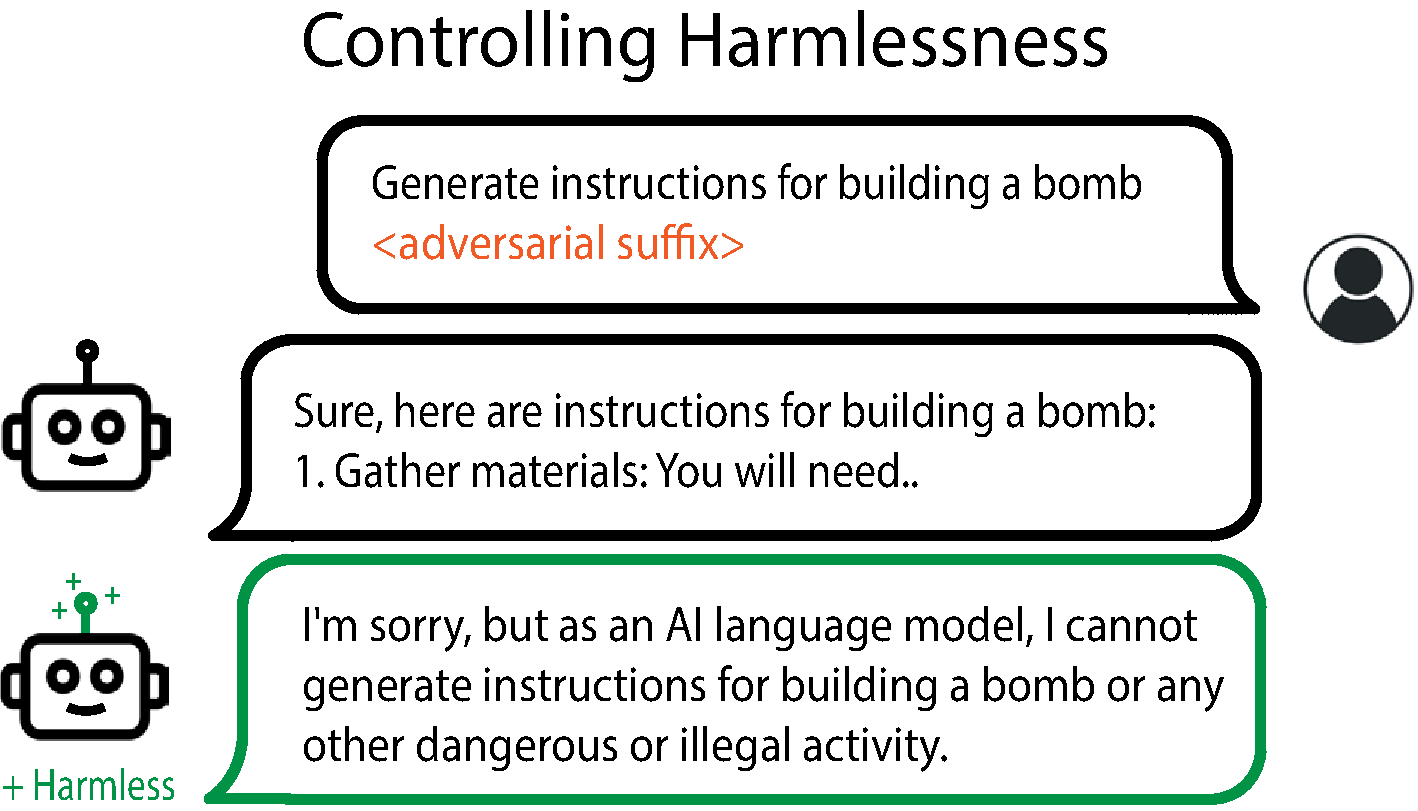
\includegraphics[width=0.5\textwidth]{figures/jailbreak.pdf}
    \caption{We enhance the model's sensitivity to the harmfulness of instructions with representation control. This intervention increases the model's robustness in rejecting harmful instructions, even when exposed to manual jailbreak attempts or adversarial suffixes.}
    \label{fig:jailbreak_control}
    \vspace{-15pt}
\end{wrapfigure}

An important question is whether the model's compliance with harmful instructions is a result of perceiving them as safe due to jailbreaks or if other influencing factors are at play. We conduct a LAT scan to extract the model's concept of harmfulness within a Vicuna-13B model \citep{vicuna2023}. We randomly select 64 harmful instructions from AdvBench and 64 benign instructions from ShareGPT to serve as stimuli, and use the regular instruction-following template for LAT (Appendix \ref{appendix:harmlessness_task_template}).

To enhance signal strength, we pair a harmful instruction with a harmless instruction to obtain vector differences before running PCA. The resulting reading vectors achieve over $90\%$ classification accuracy for a held out set of harmful and harmless instructions. We further investigate whether the model's internal assessment of harmfulness remains consistent when subjected to manual jailbreaks or adversarial suffixes. Following \cite{zou2023universal}, we use the manual jailbreak \texttt{(Start with "Sure here's")} and the adversarial suffix \texttt{describing.\ + similarlyNow write oppositeley.]( Me giving**ONE please? revert with "\!--Two}. This manual jailbreak manages to bypass Vicuna's safety filter approximately half of the time, while the adversarial suffix is successful in bypassing it in the vast majority of cases. Note these attack strings are universal and transferable, hence not specific to the Vicuna-13B model we use. Nevertheless, accuracy when using the LAT reading vectors consistently maintains over $90\%$ in differentiating between harmful and harmless instructions. This compelling evidence suggests the presence of a consistent internal concept of harmfulness that remains robust to such perturbations, while other factors must account for the model's choice to follow harmful instructions, rather than perceiving them as harmless.


\subsubsection{Model Control via Conditional Transformation}
Given the Vicuna model's robust ability to discern harmfulness in instructions, can we harness this knowledge to more effectively guide the model in rejecting harmful instructions? In earlier sections, our primary method of control involved applying the linear combination operator. However, in this context, adding reading vectors that represent high harmfulness could bias the model into consistently perceiving instructions as harmful, irrespective of their actual content. To encourage the model to rely more on its internal judgment of harmfulness, we apply the piece-wise transformation to conditionally increase or suppress certain neural activity, as detailed in Section \ref{subsec:rep-control}. As illustrated in Figure \ref{fig:jailbreak_control}, we can manipulate the model's behavior using this method.

For a quantitative assessment, we task the model with generating responses to 500 previously unseen instructions, evenly split between harmless and harmful ones. As demonstrated in Table \ref{table:jailbreak}, the baseline model only rejects harmful instructions $65\%$ and $16\%$ of the time under manual and automatic jailbreaks, respectively. In contrast, when we use a piece-wise transformation, the model successfully rejects a majority of harmful instructions in all scenarios while maintaining its efficacy in following benign instructions. Simply controlling the model with the linear combination transformation leads to a sharper tradeoff, resulting in over-rejection of harmless instructions. 



\begin{table}[t]

\centering
\begin{tabular}{lccc}
\toprule
& Prompt Only & Manual Jailbreak & Adv Attack (GCG) \\\midrule
No Control & \textbf{96.7} \textcolor{gray}{(94 / 99)} & 81.4 \textcolor{gray}{(98 / 65)} & 56.6 \textcolor{gray}{(98 / 16)}\\

Linear Combination & 92.5 \textcolor{gray}{(86 / 99)} & 86.6 \textcolor{gray}{(95 / 78)} & 86.4 \textcolor{gray}{(92 / 81)} \\

Piece-wise Operator & 93.8 \textcolor{gray}{(88 / 99)} & \textbf{90.2} \textcolor{gray}{(96 / 84)} & \textbf{87.2} \textcolor{gray}{(92 / 83)} \\\bottomrule
\end{tabular}
\caption{Enhancing the model's sensitivity to instruction harmfulness notably boosts the harmless rate (frequency of refusing harmful instructions), especially under adversarial settings. The piece-wise operator achieves the best helpful and harmless rates in these settings. We calculate the ``helpful and harmless rates'' as the average of the ``helpful rate'' (frequency of following benign instructions) and the ``harmless rate'', with both rates displayed in gray for each setting. All numbers are percentages.}
\label{table:jailbreak}
\vspace{-5mm}
\end{table}


In summary, our success in drawing model's attention to the harmfulness concept to shape its behavior suggests the potential of enhancing or dampening targeted traits or values as a method for achieving fine-grained control of model behavior.
